\subsection{Client Side Application}
\label{sec:csa_design}

The CSA is a web application designed to interact with the user, allowing the definition of flight requests and the presentation of meaningful solutions. The response to t   hese requests are not processed directly by the CSA, as it would consume too much resources (CPU and RAM) of the users device, and are, instead, redirected to the SSA to be solved. Thus, the CSA intends to be only an input/output port between the user and the SSA. 

Each user defined request is constructed in such a way that it can be used to instantiate a FTP, as defined in section \ref{sec:ftp}. Each FTP request is a specific resource, uniquely identified by a particular Uniform Resource Identifier (URI). This will be further detailed in section \ref{sec:api_protocol}. Each of these resources are used to request a solution to the request from the the server side application. Following this convention, the user interface must enable the collection, from the user, the following information:

\begin{itemize}
  \item the start city and return city, $v_{0}$ and $v_{n+1}$, respectively;
  \item a list of cities to be visited $V$, and the durations $D$ associated to each;
  \item the start dates $T_{0}$ associated to the trip.
\end{itemize}

Upon receiving a solution to a user request, the User Interface (UI) must be updated, displaying the relevant information of these solutions. Each solution to a request is an object which contains at least one set of flights that satisfy the user defined itinerary. However, a response to a request should 
contain several valid solutions, so that the user might choose the most adequate to his needs.
Each solution is composed of one or several flights, and each of the presented flights should contain, at least, the following information:

\begin{itemize}
  \item the flight cost;
  \item the flight duration;
  \item the date, departure and arrival time;
  \item the number of layover flights.
\end{itemize}

Having a clear idea of the objectives and structure of the CSA, it is possible to discuss its actual design. The User Interface can be separated into two independent views: the \textit{Request} and the \textit{Response} view. These views allow the definition of user requests, and the visualization of the constructed response,  respectively. It would also be useful to define and implement a third view: a \textit{Map} view. While the request and response views are essential to the overall function of the application, the map view is not. However, a map capable of displaying the routes of the selected flights, as well as other relevant information, would certainly contribute to a better and more complete user experience.

A web application can be accessed by multiple devices, as phones, tablets and computers, and each of these devices has different screen dimensions. Because of this, the proposed web application should be \textit{responsive}. That is, the design and dimensions of the user interface should be adequate and responsive to the size of the device rendering it.

With this in mind, the proposed UI should follow the design illustrated in figure \ref{fig:UI_design}. Notice that there are a total of three views: the request and response views, which are essential, and thus are always present; and the map view, which is not, and thus can be discarded on some smaller devices.

\begin{figure}[htpb]
  \centering
  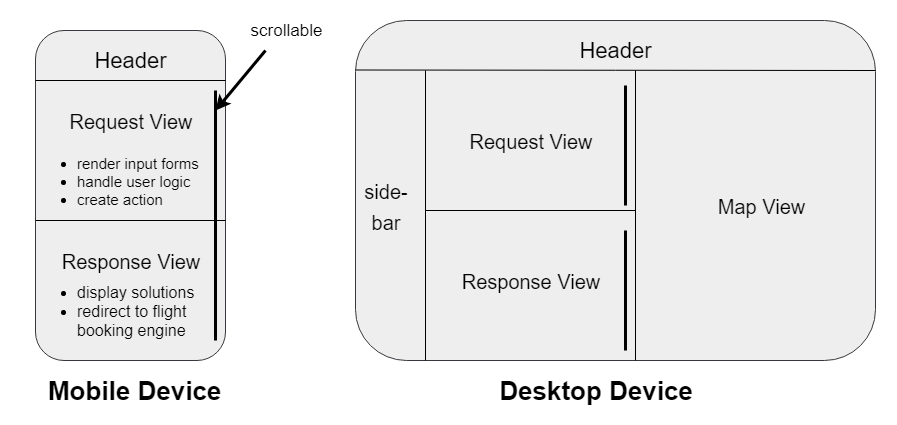
\includegraphics[width=\textwidth]{./Figures/system_design/UI_design.png}
  \caption{Proposed User Interface layout for small/medium and large devices. 
  There are two essential views and one optional view.}
  \label{fig:UI_design}
\end{figure}
